\documentclass[convert={ghostscript,gsdevice=tiffg4,
outext=.tiff,density=1200}]{standalone}
    \usepackage{tikz}
    \usepackage{pgfplots}
    \usetikzlibrary{patterns}
\mathversion{bold}
\begin{document}
\Large
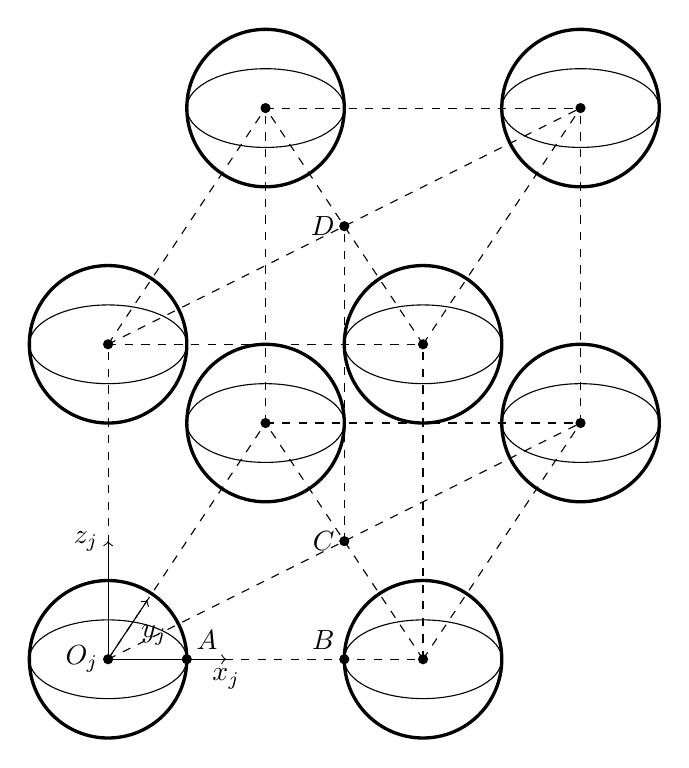
\begin{tikzpicture}%[scale=1.5]

\coordinate (O1) at (0,0);
\coordinate (O2) at (4,0);
\coordinate (O3) at (2,3);
\coordinate (O4) at (6,3);
\coordinate (O5) at (0,4);
\coordinate (O6) at (4,4);
\coordinate (O7) at (2,7);
\coordinate (O8) at (6,7);
%\coordinate (O9) at (4,4.5);
\coordinate (A) at (1,0);
\coordinate (B) at (3,0);
\coordinate (C) at (3,1.5);
\coordinate (D) at (3,5.5);

\draw[->] (0,0) -- (1.5,0) node[anchor=north] {$x_j$};
\draw[->] (0,0) -- (0,1.5) node[anchor=east] {$z_j$};
\draw[->] (0,0) -- (0.5,0.75) node[anchor=north] {};
\node[right] at (0.3,0.3) {$y_j$};

\node[left] at (O1) {$O_j$};
\node[above right] at (A) {$A$};
\node[above left] at (B) {$B$};
\node[left] at (C) {$C$};
\node[left] at (D) {$D$};

\draw[very thick] (O1) circle (1.0);
\draw (O1) ellipse (1.0 and .5);

\draw[very thick] (O2) circle (1.0);
\draw (O2) ellipse (1.0 and .5);

\draw[very thick] (O3) circle (1.0);
\draw (O3) ellipse (1.0 and .5);

\draw[very thick] (O4) circle (1.0);
\draw (O4) ellipse (1.0 and .5);

\draw[very thick] (O5) circle (1.0);
\draw (O5) ellipse (1.0 and .5);

\draw[very thick] (O6) circle (1.0);
\draw (O6) ellipse (1.0 and .5);

\draw[very thick] (O7) circle (1.0);
\draw (O7) ellipse (1.0 and .5);

\draw[very thick] (O8) circle (1.0);
\draw (O8) ellipse (1.0 and .5);

%\draw[very thick] (O9) circle (1.0);
%\draw (O9) ellipse (1.0 and .5);

\draw[dashed] (O1) -- (O2);
\draw[dashed] (O1) -- (O5);
\draw[dashed] (O1) -- (O3);
\draw[dashed] (O2) -- (O4);
\draw[dashed] (O2) -- (O6);
\draw[dashed] (O3) -- (O4);
\draw[dashed] (O3) -- (O7);
\draw[dashed] (O4) -- (O8);
\draw[dashed] (O5) -- (O6);
\draw[dashed] (O5) -- (O7);
\draw[dashed] (O6) -- (O8);
\draw[dashed] (O7) -- (O8);
\draw[dashed] (O1) -- (O4);
\draw[dashed] (O2) -- (O3);
\draw[dashed] (O5) -- (O8);
\draw[dashed] (O6) -- (O7);
\draw[dashed] (C) -- (D);

\node[circle, fill=black, inner sep=1.3pt] at (O1) {};
\node[circle, fill=black, inner sep=1.3pt] at (O2) {};
\node[circle, fill=black, inner sep=1.3pt] at (O3) {};
\node[circle, fill=black, inner sep=1.3pt] at (O4) {};
\node[circle, fill=black, inner sep=1.3pt] at (O5) {};
\node[circle, fill=black, inner sep=1.3pt] at (O6) {};
\node[circle, fill=black, inner sep=1.3pt] at (O7) {};
\node[circle, fill=black, inner sep=1.3pt] at (O8) {};
%\node[circle, fill=black, inner sep=1.3pt] at (O9) {};
\node[circle, fill=black, inner sep=1.3pt] at (A) {};
\node[circle, fill=black, inner sep=1.3pt] at (B) {};
\node[circle, fill=black, inner sep=1.3pt] at (C) {};
\node[circle, fill=black, inner sep=1.3pt] at (D) {};

\end{tikzpicture}
\end{document}

%%% Local Variables: 
%%% mode: latex
%%% TeX-master: t
%%% End: 
